
%\setcounter{page}{45}
\clearpage
%\pagenumbering{arabic}
\newpage
% \addcontentsline{toc}{chapter}{\hfill 34}
\addtocontents{toc}{\protect\contentsline{chapter}{CAPÍTULO IV. Propuesta de diseño   \hfill  83}{}{}}






\begin{titlepage}
	
	
	\centering
	\begin{tikzpicture}%opacity=0.5
		\node[inner sep=0pt, ] (image) at (0,0) {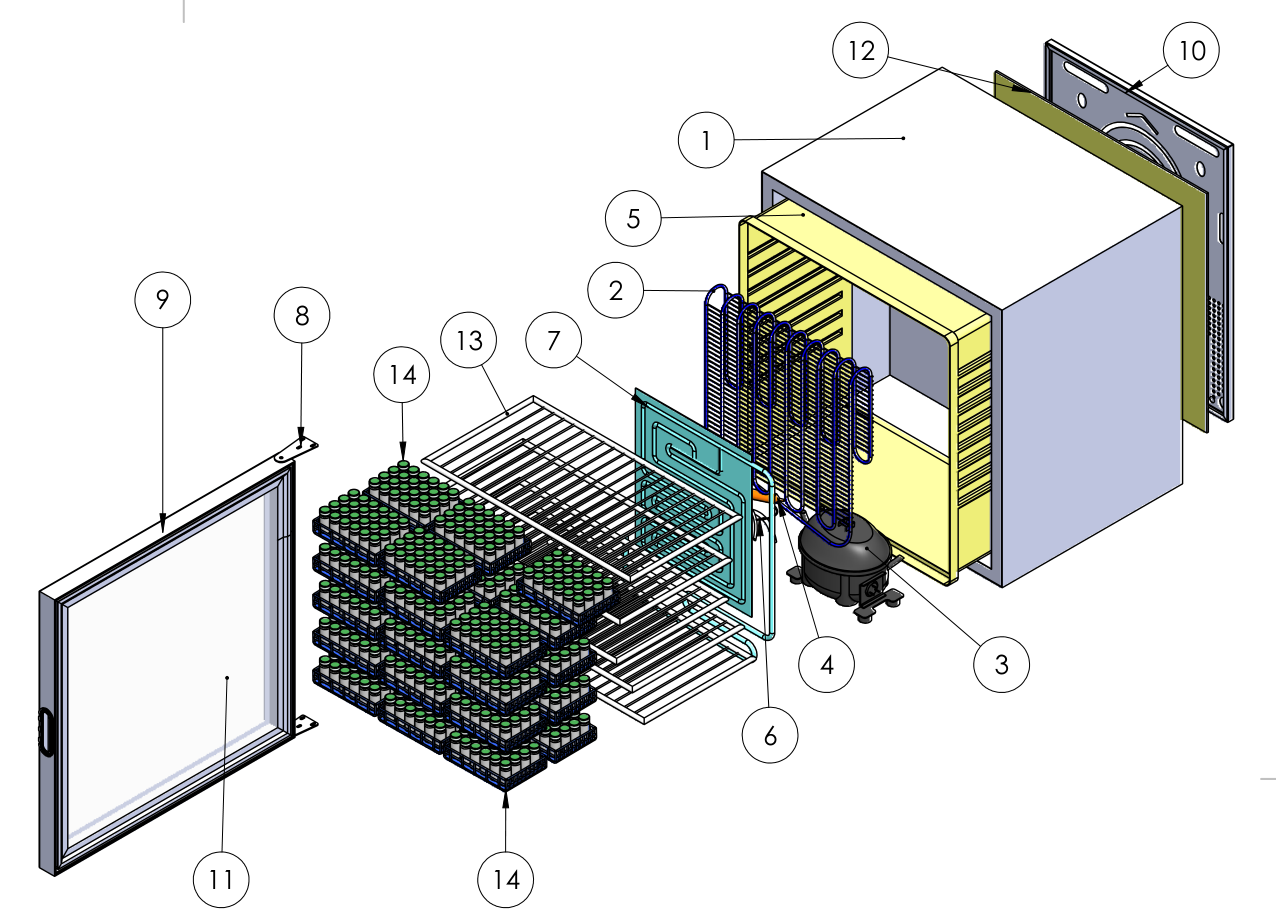
\includegraphics[width=\textwidth]{figures/front-chapetr4}};
		\fill [white,path fading=south] (-5,-4) rectangle (5,4);
		\node[black,font=\Huge\bfseries] at (0,3) {Capítulo IV. Propuesta de diseño};
		\node[black,font=\Large\bfseries] at (0,1) {Cálculo térmico y selección de componentes};
		\node[black,font=\Large\bfseries] at (0,0) {Diseño de propuesta en SolidWorks};
	\end{tikzpicture}
\end{titlepage}


 \newpage 
 
 \section*{Introducción}
 
 
 \addcontentsline{toc}{section}{{Introducción}} 
 \setcounter{chapter}{4}
 \setcounter{page}{84}   
 \setcounter{section}{0}
 \setcounter{figure}{0}
 \setcounter{table}{0}
 
 El núcleo de la investigación reside en la aplicación de la teoría físico-matemática, particularmente en los aspectos técnicos que involucran el cálculo de cada componente del sistema, así como sus parámetros fundamentales. Estos cálculos, producto de años de investigación, son esenciales para asegurar la correcta funcionalidad del equipo de refrigeración seleccionado.\\
 Para optimizar la distribución de los elementos del sistema, se calculan las cargas térmicas con base en tablas y gráficos científicos especializados en refrigeración. Esto nos permite seleccionar el equipo adecuado y diseñar un sistema que cumpla con las necesidades específicas del proyecto. Los antecedentes del lugar donde se instalará la cámara de refrigeración proporcionan información crucial para identificar las condiciones críticas a las que estará expuesta, como la temperatura ambiente y las posibles fuentes de calor externas.\\
 El cálculo preciso de las propiedades térmicas de la insulina y su entorno es esencial. Esto incluye no solo la temperatura de almacenamiento, sino también el material de la cámara de transporte y el acomodo óptimo del producto para minimizar la transferencia de calor desde el exterior. Estas propiedades, determinadas experimentalmente, nos proporcionan los datos necesarios para realizar los ajustes pertinentes en el diseño.\\
 Finalmente, se realizan las modificaciones necesarias al diseño inicial, que se propuso en el capítulo III (MetaDiseño), del semestre anterior, tomando en cuenta cualquier cambio surgido durante el proceso de cálculo y distribución del equipo. El resultado es una propuesta final que se presenta con planos detallados de las dimensiones del sistema, garantizando una funcionalidad eficiente y segura para la conservación de la insulina.\\
En los capítulos previos se establecen las bases fundamentales   para la comprensión del diseño térmico y de cámaras de conservación de insulina, así como el contexto específico del proyecto. En el \textbf{Capítulo 1}, se abordan las generalidades del diseño térmico, con especial atención a los principios físicos y matemáticos que rigen los sistemas de refrigeración, conocimientos esenciales estudiados en la \textit{Escuela Superior de Ingeniería Mecánica y Eléctrica} (ESIME) del \textit{Instituto Politécnico Nacional}. El \textbf{Capítulo 2} contextualiza el proyecto, ofreciendo una visión clara sobre la necesidad y relevancia de la conservación de insulina en clínicas como la UMF 40 en Azcapotzalco. Por último, el \textbf{Capítulo 3} se enfoca en el metadiseño, donde se presentan los lineamientos y directrices que guiarán la implementación técnica del sistema de refrigeración, fundamentados en los temas estudiados en ESIME, tales como el análisis de cargas térmicas y la selección de equipos especializados.
 \newpage
\section{Marco referencial}\rspitems
\subsection{Normas ISO en planos de ingeniería}
Basarse en normas ISO es fundamental para los proyectos de ingeniería, ya que estas normas proporcionan un marco reconocido internacionalmente que garantiza la calidad, seguridad y compatibilidad de los diseños. En particular, para el diseño de equipos de refrigeración médica, el cumplimiento de estas normas es esencial para asegurar que los sistemas funcionen de manera óptima y cumplan con los requisitos de conservación de productos sensibles, como la insulina. Las normas ISO permiten que los diseños sigan un estándar riguroso, lo que facilita la colaboración entre equipos internacionales y asegura que los productos cumplan con las exigencias de seguridad y eficacia del sector.\rspitems
\subsubsection{Norma ISO 5457 (Presentación de dibujos técnicos) }\rspitems
La Norma ISO 5457 es un estándar internacional que proporciona directrices para la presentación de dibujos técnicos en papel y en formato digital. Esta norma define los tamaños de papel, los márgenes, las líneas y las convenciones de representación gráfica, entre otros aspectos, con el objetivo de garantizar la legibilidad y la claridad de los dibujos técnicos \cite{manzanelli-2023}.\rspitems
\subsubsection{Norma ISO 6433:2012 (Documentación técnica del producto)}\rspitems
Esta Norma Internacional proporciona reglas para la presentación de referencias de piezas en representaciones de conjuntos. Por ejemplo, en dibujos de conjunto, para identificar las partes constituyentes en una lista de partes relacionadas \cite{iso_org-2024}.
También se toman las siguientes recomendaciones con el titular de la materia del proyecto 2, el Dr.  \citeauthor{sotomucino2024}, durante el curso 25/1.
\begin{enumerate}
	\item A cada pieza del conjunto se le debe asignar una marca única que sirva como referencia del elemento. Esta marca debe diferenciarse claramente de cualquier otra indicación presente en el dibujo.\rspitems	
	\item Los elementos idénticos dentro de un conjunto deben identificarse con la misma referencia, y si no hay riesgo de ambigüedad, se mencionarán únicamente una vez.	\rspitems
	\item En caso de que existan grupos de elementos, cada subconjunto debe recibir una referencia única que lo identifique.\rspitems
	\item Cada referencia debe estar conectada visualmente con el elemento correspondiente mediante una línea de referencia, que se extienda desde la marca hasta un punto o una flecha, de acuerdo con los principios generales de representación gráfica establecidos en los dibujos técnicos.\rspitems
	\item Las referencias deben colocarse de manera que garanticen la máxima claridad y legibilidad del dibujo, preferiblemente organizadas en filas y columnas alineadas.\rspitems
	\item El orden para numerar las referencias debe seguir un criterio definido, como por ejemplo:
	\begin{itemize}
		\item Orden de montaje posible.\rspitems
		\item Orden de importancia de los elementos.\rspitems
		\item Cualquier otro criterio lógico que se ajuste a las necesidades del diseño.\rspitems
	\end{itemize}
\end{enumerate}\rsp
\subsubsection{ISO 7573:2008 (Listas de piezas):}\rspitems
La norma ISO 7573:2008 establece los requisitos mínimos que deben cumplir las listas de piezas para proporcionar la información necesaria, por ejemplo, para la producción, la adquisición o el mantenimiento de las piezas. Abarca tanto las listas de piezas manuales como las generadas por ordenador.

 
 \section{Propuesta solución}

 
Considerando el objetivo del proyecto, que se centra en el almacenamiento para la conservación de insulina, partimos de la necesidad de la Unidad de Medicina Familiar (UMF 40) y de las clínicas ubicadas en un radio de 1 kilómetro, para garantizar el abastecimiento de este medicamento en la alcaldía Azcapotzalco, Ciudad de México. Actualmente, la UMF 40 cuenta con una sola cámara de refrigeración, diseñada según los estándares de los principales fabricantes en el mercado de la refrigeración médica. Sin embargo, esta cámara se utiliza para almacenar al menos tres tipos de medicamentos, lo que genera problemas relacionados con la seguridad y eficiencia en el manejo de los mismos. Por tanto, el propósito del proyecto es realizar un cálculo preciso de la carga energética y térmica, considerando todos los factores que pueden influir en la localización, recepción y manejo del medicamento. Esto permitirá asegurar un óptimo funcionamiento del equipo, reducir el consumo energético y evitar la adquisición de equipo innecesario, garantizando la calidad y efectividad de la insulina antes de su administración.\\
Las dimensiones de la Cámara Frigorífica fueron tomadas de acuerdo con la demanda, espacio disponible en el área de farmacia y flujo de recepción del producto que se presenta a los pacientes de la alcaldía. La insulina llega en cajas de plástico por paquetes, donde estás pasan un proceso de control de calidad y sanidad por personal especializado de la UMF 40, después se montan en charolas o plásticos comunes y corrientes (una mala práctica que se planea erradicar), con el fin de distribuir el medicamento en algún compartimento del refrigerador libre y etiquetar el medicamento de acuerdo a los lineamientos del hospital regidos por el IMSS.\\
La distribución de la cámara de refrigeración se detalla en la figura \ref{fig:4-propuestasol}. El contenedor del refrigerador está adaptado con láminas compuestas de poliuretano (película interna $f_i$ - Poliuretano - película externa $f_e$) en las cuatro paredes, con el objetivo de minimizar la pérdida de temperatura por transferencia térmica a través de las superficies. Esta aislación contribuye a evitar el uso de ventiladores, mejorando la eficiencia energética en las etapas iniciales del funcionamiento.\\
En la parte posterior de la cámara se integra la unidad de refrigeración, cuya función es proteger los componentes del sistema. Esta unidad alberga los elementos principales, como el compresor, el condensador y el dispositivo de expansión, que están conectados directamente al evaporador. El evaporador está situado en el interior de la cámara y conectado al serpentín, cuya función es asegurar una mejor distribución del refrigerante dentro de la cámara, lo que permite una disipación de calor más eficiente y uniforme.\\
Además, la cámara está equipada con diversas tapas y una cubierta de cristal, diseñadas para mantener el medicamento en condiciones óptimas de almacenamiento.
  
  \begin{figure}[H]
 	\centering
 	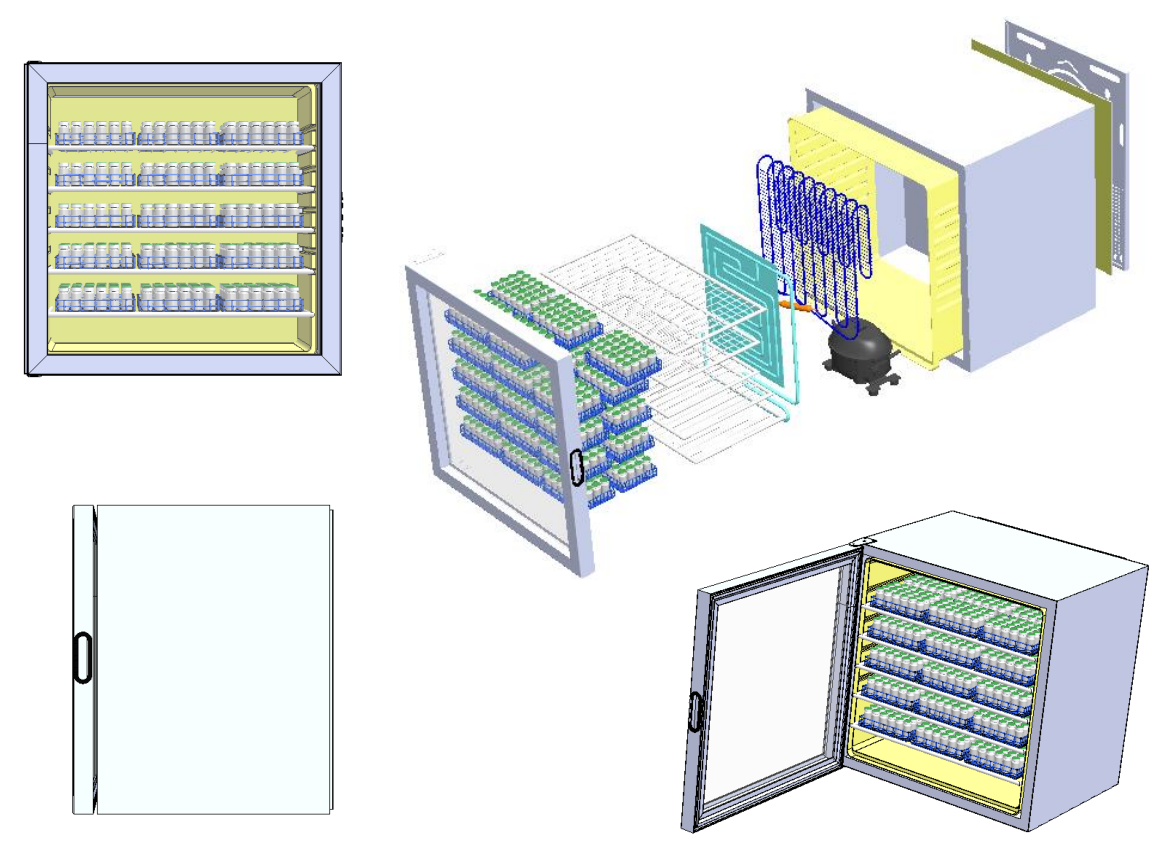
\includegraphics[width=0.8\linewidth]{figures/4-propuesta_sol}
 	\caption{Vistas de la cámara de refrigeración.}
 	Fuente: Elaboración propia usando \texttt{SolidWorks.}
 	\label{fig:4-propuestasol}
 \end{figure}
 
 \subsubsection{Unidad de refrigeración}
Como se muestra en la figura \ref{fig:4-coolerunit}, se ha dispuesto que la unidad de refrigeración se ubique en la parte trasera y exterior de la cámara de refrigeración. Esta elección es fundamental, ya que la unidad genera calor durante su operación, lo que, de no estar adecuadamente posicionada, podría elevar la temperatura interna de la cámara. Tal incremento de temperatura es crítico, ya que puede comprometer la integridad y efectividad de la insulina, que requiere condiciones específicas de almacenamiento para garantizar su estabilidad y seguridad.\\
La unidad de refrigeración alberga componentes esenciales del sistema, como el condensador, el compresor y la válvula de expansión. Cada uno de estos elementos desempeña un papel crucial en el ciclo de refrigeración. El compresor, por ejemplo, es responsable de comprimir el refrigerante, aumentando su presión y temperatura, mientras que el condensador permite que el refrigerante se enfríe y se condense, liberando el calor hacia el ambiente. La válvula de expansión regula el flujo del refrigerante hacia el evaporador, donde se produce la refrigeración efectiva del aire dentro de la cámara.\\
La adecuada ubicación y el funcionamiento eficiente de esta unidad son vitales para mantener un ambiente controlado en el interior de la cámara, garantizando así que la insulina se conserve en condiciones óptimas, protegiendo su eficacia y, en última instancia, la salud de los pacientes que dependen de este tratamiento.
 
 \begin{figure}[H]
 	\centering
 	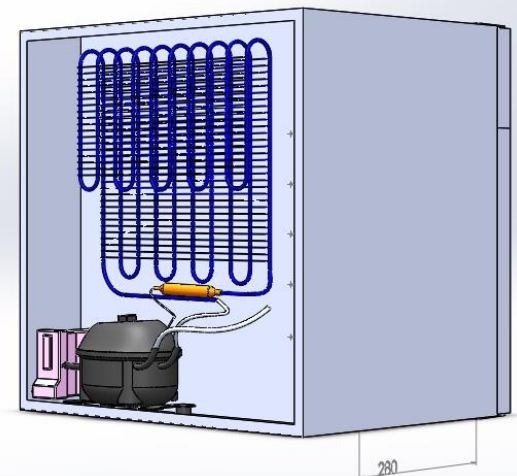
\includegraphics[width=0.4\linewidth]{figures/4-cooler_unit}
 	\caption{Unidad de refrigeración.}
 	Fuente: Elaboración propia usando \texttt{SolidWorks.}
 	\label{fig:4-coolerunit}
 \end{figure}
  
 \subsubsection{Evaporador}
 
 
En la figura \ref{fig:4-evaporator}, el evaporador del sistema se ubica en la parte interior de la cámara, proporcionando un espacio de almacenamiento adecuado y una posición estratégica que optimiza su rendimiento. El evaporador está diseñado con un serpentín que se seleccionará en función de varios factores, como la carga térmica esperada, el tipo de refrigerante utilizado y las características específicas de la insulina a conservar. \\
Dado que la cámara tiene dimensiones de $60\times 60 \times 51{.}2$ centímetros, es fundamental considerar aspectos como el flujo de aire interno y la distribución térmica. La selección del serpentín garantizará una transferencia de calor eficiente y uniforme, minimizando las zonas frías o calientes que podrían afectar la integridad del producto. Además, en los cálculos de secciones posteriores se considera, la capacidad del evaporador para manejar la carga térmica en función de la cantidad y tipo de insulina almacenada, así como las condiciones ambientales externas propias de la Alcaldía. 
 \begin{figure}[H]
 	\centering
 	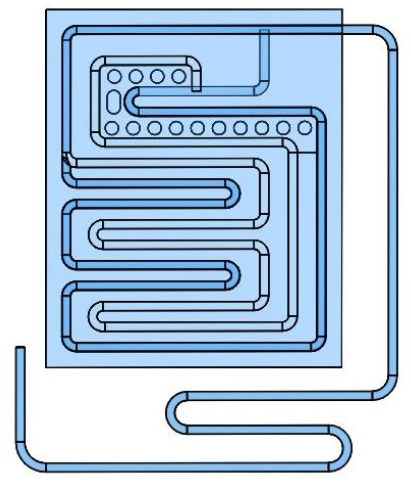
\includegraphics[width=0.4\linewidth]{figures/4-evaporator}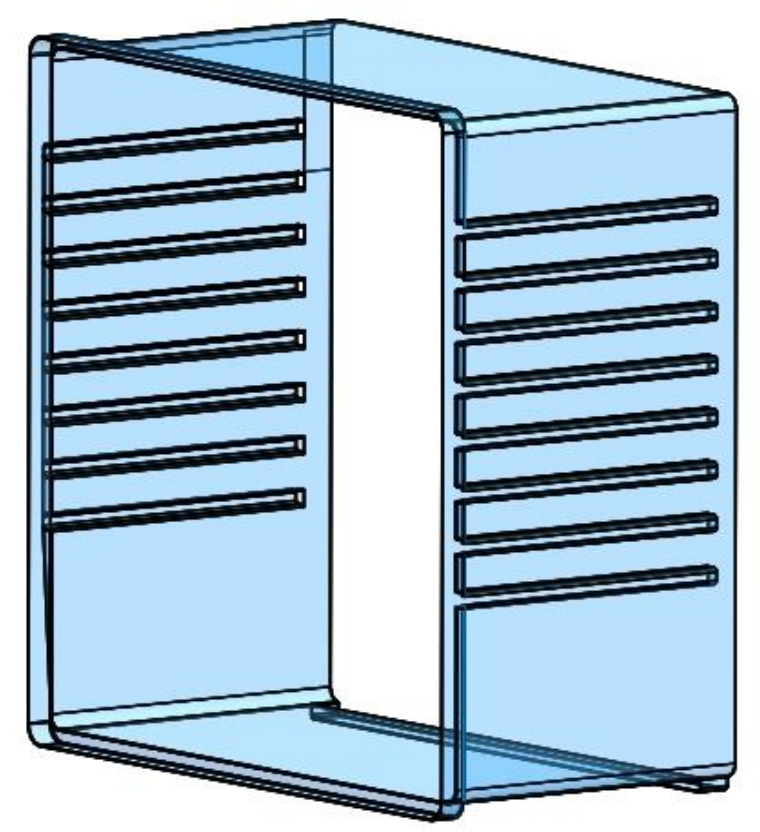
\includegraphics[width=0.4\linewidth]{figures/4-evaporator2}
 	\caption{Vistas del evaporador (serpentín).}
 	Fuente: Elaboración propia usando \texttt{SolidWorks.}
 	\label{fig:4-evaporator}
 \end{figure}\rsp 
 
 \subsubsection{Serpentín del condensador}
 El serpentín del condensador de la figura  \ref{fig:4condenser}, es una parte fundamental del sistema de refrigeración, cuya función principal es la de disipar el calor absorbido por el refrigerante durante su ciclo de compresión. En el contexto de la conservación de insulina, la correcta operación del serpentín es crítica para mantener la temperatura interna de la cámara en niveles óptimos. El serpentín del condensador se ubica en la parte externa de la cámara de refrigeración para asegurar que el calor no regrese al compartimento donde se almacena la insulina.\\
 Una mala selección o una disposición ineficiente del serpentín podría resultar en una refrigeración inadecuada, generando fluctuaciones de temperatura que comprometerían la estabilidad del medicamento. Mantener una temperatura constante es crucial para la preservación de la insulina, ya que cambios bruscos pueden degradar su eficacia.
 \begin{figure}[H]
 	\centering
 	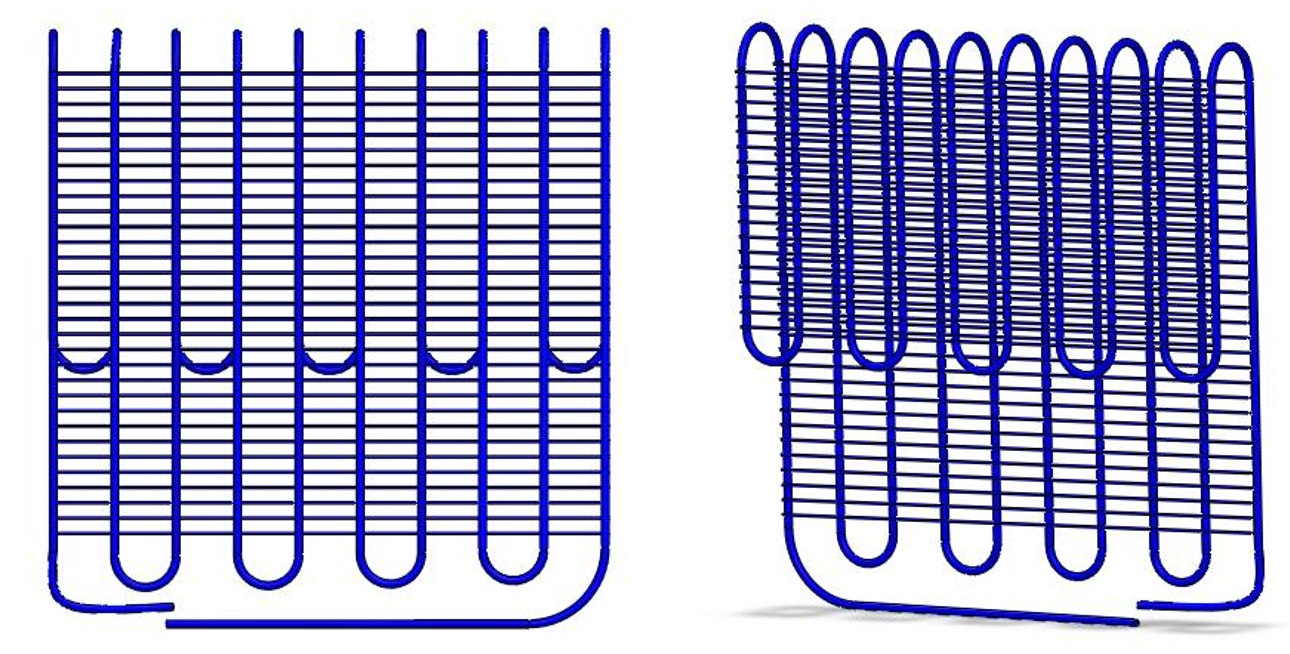
\includegraphics[width=0.6\linewidth]{figures/4condenser}
 	\caption{Vista del serpentín del condensador}
 	Fuente: Elaboración propia usando \texttt{SolidWorks.}
 	\label{fig:4condenser}
 \end{figure}
 
 
 \subsubsection{Compresor}
 En la figura \ref{fig:4-compressor}, el compresor del sistema se localiza en la parte externa de la cámara de refrigeración, siendo una de las piezas clave para el funcionamiento eficiente del sistema. Este componente es responsable de aumentar la presión del refrigerante, permitiendo su circulación a través del sistema de refrigeración y garantizando que el evaporador reciba el refrigerante en condiciones óptimas. \
 
 Para la selección del compresor, se tomarán en cuenta varios factores, tales como la carga térmica requerida para conservar la insulina, la eficiencia energética y el tipo de refrigerante utilizado. Es esencial que el compresor cuente con la capacidad suficiente para manejar la carga térmica, asegurando un funcionamiento constante y eficiente, especialmente considerando las variaciones de temperatura en la Alcaldía de Azcapotzalco. \
 
 Además, se evaluará la compatibilidad del compresor con el sistema de control de temperatura de la cámara, ya que un control adecuado es crucial para mantener las condiciones óptimas para la conservación de la insulina. La elección de un compresor eficiente no solo contribuirá a un menor consumo energético, sino que también asegurará la integridad y efectividad del medicamento almacenado.
 
 \begin{figure}[H] 
 	\centering 
 	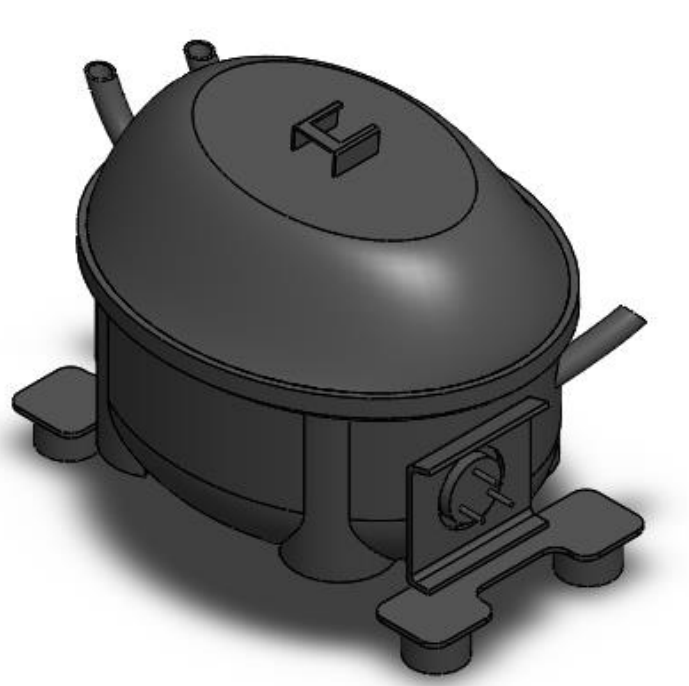
\includegraphics[width=0.4\linewidth]{figures/4-compressor}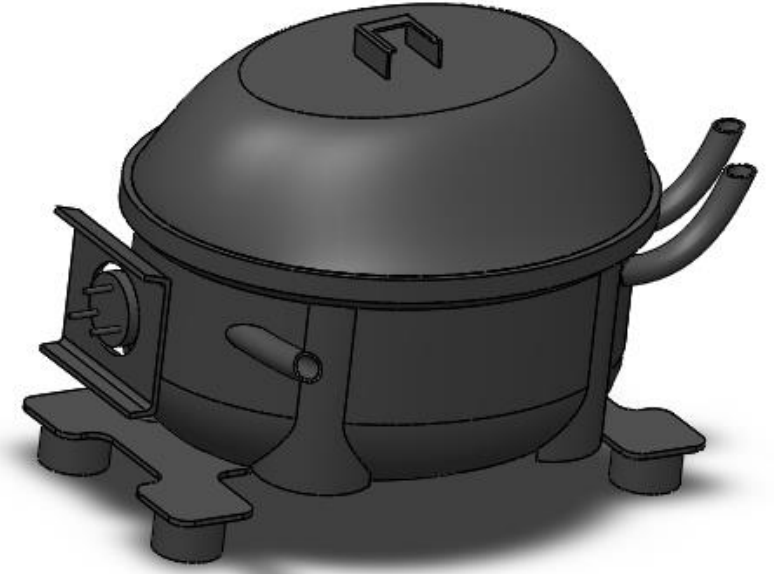
\includegraphics[width=0.4\linewidth]{figures/4-compressor2}
 	\caption{Vistas del compresor.} 
 	Fuente: Elaboración propia usando \texttt{SolidWorks.} 
 	\label{fig:4-compressor}
 \end{figure}
 
\subsubsection{Válvulas de expansión}
En la figura \ref{fig:4-expvalves} se muestra la válvula de expansión de nuestro sistema, éstas válvulas juegan un rol indispensable en el sistema de refrigeración, ya que controlan el flujo de refrigerante hacia el evaporador, permitiendo que el refrigerante se expanda y disminuya su temperatura antes de entrar en contacto con la cámara interna. En este caso, la válvula de expansión debe estar calibrada con precisión para mantener la temperatura estable en el rango adecuado para la conservación de insulina, que como ya sabemos está típicamente entre 2 °C y 8 °C.

\begin{figure}[H]
	\centering
	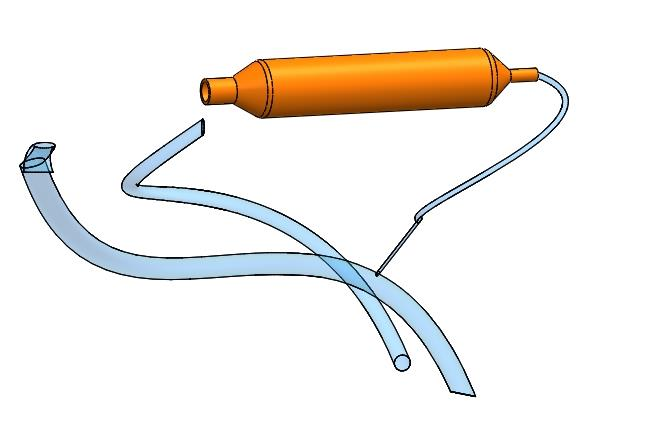
\includegraphics[width=0.5\linewidth]{figures/4-expvalves}
	\caption{Vista de las válvulas de expansión}
	Fuente: Elaboración propia usando \texttt{SolidWorks.}
	\label{fig:4-expvalves}
\end{figure}


\subsection{Esquema de bloques del funcionamiento del sistema}
 
 \begin{figure}[H]
 \centering 
  \begin{tikzpicture}[node distance=2cm and 1cm]
  	
  	% Bloques del sistema
  	\node (input) [block] {Entrada de potencia};
  	\node (compressor) [block, right=of input] {Compresor};
  	\node (condenser) [block, right=of compressor] {Condensador};
  	
  	% Filtro de secado más abajo
  	\node (filter) [block, below=of condenser] {Filtro de Secado};
  	\node (evaporator) [block, left=of filter] {Evaporador};
  	\node (valve) [block, left=of evaporator] {Válvula de Expansión};
  	\node (output) [block, left=of valve] {Salida de potencia};
  	
  	% Flechas entre los bloques
  	\draw [arrow] (input) -- (compressor);
  	\draw [arrow] (compressor) -- (condenser);
  	
  	% Flecha hacia abajo
  	\draw [arrow] (condenser) -- (filter);
  	
  	% Flecha de vuelta a la izquierda
  	\draw [arrow] (filter) -- (evaporator);
  	\draw [arrow] (evaporator) -- (valve);
  	\draw [arrow] (valve) -- (output);
  	
  \end{tikzpicture}
 \caption{Esquema de bloques del funcionamiento del sistema.}
 Fuente: Elaboración propia usando \texttt{Tikz}.
 \label{fig:4-blocksche}
\end{figure} 
  Este esquema, figura \ref{fig:4-blocksche}, ilustra el funcionamiento de un sistema de refrigeración, mostrando cada uno de los componentes clave y su rol en el proceso. A continuación, se explica cada etapa:
  \begin{enumerate}
 \item Entrada de potencia: Es la fuente de energía que alimenta el sistema. En la mayoría de los casos, esta energía es eléctrica, aunque en algunos sistemas puede ser mecánica. Es necesaria para que todos los componentes del sistema funcionen correctamente.
  
 \item Compresor: Este componente es esencial, ya que comprime el refrigerante (que en este caso suele ser un gas). Al comprimirlo, aumenta tanto la presión como la temperatura del gas, lo que es fundamental para los pasos siguientes del ciclo.
  
  \item Condensador: Una vez que el refrigerante ha sido comprimido, el condensador se encarga de disipar el calor del refrigerante caliente. El calor se libera hacia el exterior del sistema y, al perder calor, el refrigerante cambia de estado, pasando de gas a líquido.
  
 \item  Filtro de secado: Este pequeño pero importante componente tiene la tarea de eliminar cualquier traza de humedad o impureza del refrigerante líquido. Esto es vital, ya que la presencia de humedad podría dañar otros componentes del sistema, como la válvula de expansión.
   \item  Evaporador: Este es el componente donde ocurre la verdadera refrigeración. El refrigerante frío se evapora dentro del evaporador, absorbiendo el calor del área que necesita ser enfriada. Aquí, el refrigerante cambia nuevamente de líquido a gas.  
 \item  Válvula de expansión: Una vez que el refrigerante ha sido filtrado, la válvula de expansión regula el flujo de refrigerante que entra al evaporador. Además, reduce la presión del refrigerante, lo que hace que se enfríe aún más antes de llegar al evaporador.
  \item  Salida de potencia: Representa la energía térmica que el refrigerante ha absorbido del espacio enfriado y que será liberada cuando el ciclo comience de nuevo en el compresor. El proceso es cíclico y continuo, manteniendo así la refrigeración estable.
 
  \end{enumerate}
  
  
\section{Antecedentes}
                                                                                                                             En esta sección del capítulo, se presenta la base teórica de los cálculos realizados, destacando las observaciones clave del proceso de análisis y selección de los parámetros más adecuados. Además, se ofrece un resumen de los manuales utilizados como referencia para los cálculos, proporcionando un contexto claro y justificado para las decisiones tomadas.\\
Como se describió en la sección \ref{sec:contex_geografico}, el contexto geográfico es fundamental para el análisis del balance térmico o energético.
\subsection{Ubicación}
Tomando en cuenta que para lograr un alto rango de efectividad es necesario considerar las condiciones críticas de cualquier parámetro relevante, en este proyecto la ubicación geográfica juega un papel fundamental. En particular, se toma como referencia el Pueblo de Santa Bárbara, en la alcaldía Azcapotzalco, Ciudad de México. Las figuras  \ref{fig:mapsumf40} a \ref{fig:calordf} muestran tanto la ubicación geográfica como las condiciones climáticas del área, las cuales se resumen a continuación (ver también el mapa general en la figura \ref{4-mexicomap}):


\begin{itemize}
	\item Temperatura de bulbo seco: 25 °C (77 °F)\rspitems
	\item Temperatura de bulbo húmedo: 20 °C (68 °F)	\rspitems
	\item Altitud: 2,240 msnm \rspitems
	\item Presión atmosférica: 1,023 Pa (1 atm)\rspitems
\end{itemize}

\begin{figure}[H]
	\centering
	\includegraphics[width=0.6\linewidth]{figures/4-mexicomap}
	\caption{Mapa de localización del municipio Santa Bárbara Azcapotzalclo en la Ciudad de México.}\cite{semovi-24}
	\label{fig:4-mexicomap}
\end{figure}

\subsection{Tipo de producto}
\textbf{Insulina}\\
De acuerdo a la información recabada en la visita a la unidad 40 del IMSS se sabe que a los pacientes diabéticos se les proporciona dos tipos de insulina para su tratamiento, \textbf{Humalog Insulina Lispro} Figura \ref{fig:lispro-insul} e \textbf{Insulina Lantus}  Figura \ref{fig:lantus-insul}, este par de medicamentos se suministran directamente por parte del gobierno por lo que la logistica del proceso en la cadena de suministro está debidamente regulada. Además visite las tablas \ref{tabla:humalog} y \ref{tabla:lantus} para más detalles descritos del producto. Un resumen de dicha información se muestra en \ref{tabla:condsinsulina}

\subsubsection{Condiciones del producto a refrigerar.}


\begin{table}[H]
	\centering
	\caption{Condiciones del producto}
	Fuente: Elaboración propia, tomando datos directamente en la UMF.40
  	\begin{tabular}{cccc}
 		\hline
 		\textbf{Producto} & \multicolumn{3}{c|}{\textbf{Condiciones de almacenamiento}}                                                                                                                                                                        \\ \hline
 		& \textbf{\begin{tabular}[c]{@{}c@{}}Temp. \\ Almacenamiento (°C)\end{tabular}} & \textbf{\begin{tabular}[c]{@{}c@{}}Humedad \\ relativa (\%)\end{tabular}} & \textbf{\begin{tabular}[c]{@{}c@{}}Vida aprox. \\ (días)\end{tabular}} \\ \hline
 		\textbf{Insulina} & \begin{tabular}[c]{@{}c@{}}2 - 8\\ (3)\end{tabular}                           & \begin{tabular}[c]{@{}c@{}}35 - 70\\ (40)\end{tabular}                    & \begin{tabular}[c]{@{}c@{}}28\\ (antes de abrir)\end{tabular}          \\ \hline
 	\end{tabular}
 \begin{tabular}{cccc}
 	\hline
 	\textbf{Producto}    & \multicolumn{3}{c|}{\textbf{Condiciones de almacenamiento}} \\
 	& \textbf{CPB}        & \textbf{CPA}        & \textbf{HL}     \\ \cline{2-4} 
 	\textbf{Insulina}    & \textbf{Btu/lb °F}  & \textbf{Btu/lb °F}  & \textbf{Btu/lb} \\
 	\multicolumn{1}{l}{} & 1                   & 0.35                & 0.2006          \\ \hline
 \end{tabular}
 	 \label{tabla:condsinsulina}
\end{table}



\subsection{Temperatura del diseño de almacenaje}
 
En todos los procesos de refrigeración, es fundamental centrarse en el producto que requiere conservación, ya que nuestro principal objetivo es asegurar que se mantenga a la temperatura adecuada. Por lo tanto, es crucial contar con información cuantitativa y cualitativa precisa sobre las condiciones óptimas de almacenaje de dicho producto para garantizar su integridad y eficacia.
 
 \subsubsection{Temperatura de almacenamiento de la Insulina}
 
 De acuerdo con los proveedores \citeauthor{lispro-2006}, \citeyear{lispro-2006} y \citeauthor{lantus-2015},\citeyear{lantus-2015}, la temperatura de almacenamiento de la insulina es un aspecto para garantizar su calidad y eficiencia a cada paciente. En los centros de distribución y almacenaje, se conservan en el refrigerador a una temperatura de 2.7°C, y en las farmacias para su distribución directa al paciente deben conservar una temperatura entre 2°C - 8°C, visite los cuadros resumen de cada marca, Humalog (\ref{tabla:humalog}) y Lantus (\ref{tabla:lantus}).
 
 \subsection{Tipo de empaque para su almacenaje}
 
Durante una entrevista realizada con el personal médico de la UMF 40, se obtuvo información sobre el manejo de insulina en el área de distribución y almacenamiento de la farmacia de la unidad. El medicamento se transporta en cajas que contienen un número determinado de frascos, según la marca, donde cada caja incluye una cantidad específica de dosis de insulina. Debido a su alta ergonomía, se han considerado charolas de almacenamiento que facilitan la organización de las dosis sin su empaque original. Este arreglo no solo optimiza el espacio disponible, sino que también permite una manipulación más ágil, especialmente en situaciones extraordinarias, como desastres naturales o fallas en los equipos de refrigeración. En la tabla \ref{tabla:almacenaje} se presentan los detalles de las charolas utilizadas para dicho almacenamiento, en breve, se usarán parrillas de acero inoxidable con charolas de plástico, que está compuesta de polietileno de alta densidad, con las dimensiones que se describen a continuación.
 \subsection{Capacidad de almacenaje}
 \begin{table}[H]
 	\centering
 	\caption{Datos de capacidad y dimensiones de los empaques de almacenaje}\rspitems Fuente: Elaboración propia
 	\begin{tabular}{ccc}
 		\hline
 		\textbf{Tipo de empaque para su almacenaje} & \textbf{Capacidad neta (kg)} & \textbf{Dimensiones (cm)} \\ \hline
 		Unidad de charolas & 2.5 kg & 20 x 20 x 3 \\  
 		30 charolas & 75 kg & 60 x 60 x 52 \\  
 		\hline
 	\end{tabular} 	
 	\label{tabla:almacenaje}
 \end{table}
 
 Se tomará en cuenta para la Cámara frigorífica un arreglo de 5 parrillas, cada parrilla
 tendrá 6 charolas, cada una con 2.4 kg de insulina más 100 gramos del peso de la charola, lo que equivale a 15 kg por parrilla, así entonces se tiene un total de 75 kg y 720 frascos.
 \begin{equation}
 \begin{aligned}
 	\text{Número de charolas} &= \dfrac{75 kg}{2.5kg} = 30 \text{charolas}\\
 		\text{Número de charolas por tarima} &= \dfrac{30\; charolas}{5\; tarimas} = 6 \text{charolas por tarima}
 \end{aligned}
\end{equation}
El fabricante nos recomienda que el apilamiento debe contener 30 kg como máximo y de acuerdo a los cálculos realizados, se está dentro de lo permitido.

\subsection{Flujo de recepción}

Hablando de un producto a refrigerar de la manera más eficiente, el caso más optimo a considerar es colocar todo el producto en el tiempo más corto posible. Flujo de recepción: 225 Kg / Día, en 3 visitas del centro de distribución del gobierno mexicano.


\subsection{Planos y diagramas}
El acomodo de las charolas puede realizarse de distintas formas. Sin embargo, es fundamental garantizar que estén colocadas de manera estable, evitando que se vuelquen o desplacen durante la administración o distribución a los pacientes. Por esta razón, se sugiere distribuirlas de forma uniforme sobre la superficie de la parrilla. A continuación, se presenta un ejemplo de cómo se apilan las charolas llenas de frascos de insulina, colocadas una sobre otra sin dejar espacios entre ellas, tal como se muestra en la figura \ref{fig:4-frontalcharolas}.


\begin{figure}[H]
	\centering
	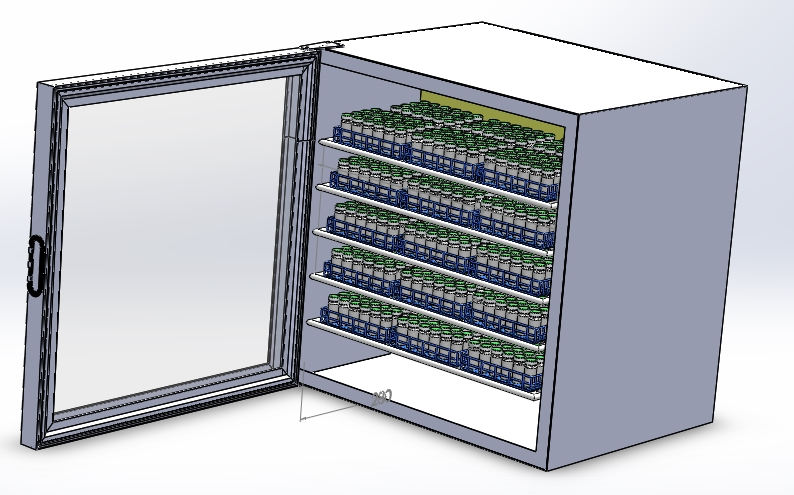
\includegraphics[width=0.6\linewidth]{figures/4-frontalcharolas}
	\caption{Vista frontal de la cámara de refrigeración llena de la insulina.}
	Fuente: Elaboración propia usando \texttt{SolidWorks.}
	\label{fig:4-frontalcharolas}
\end{figure}


En la figura \ref{fig:4-lateralcharolas1} se muestran las vistas laterales del acomodo de las charolas dentro de de la cámara de refrigeración    .

\begin{figure}[H]
	\centering
	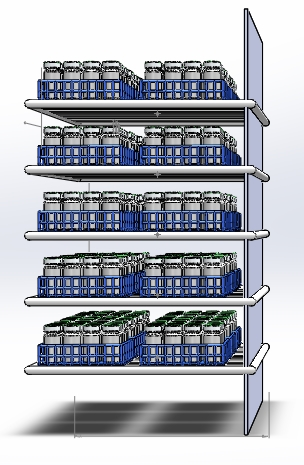
\includegraphics[width=0.4\linewidth]{figures/4-lateralcharolas1}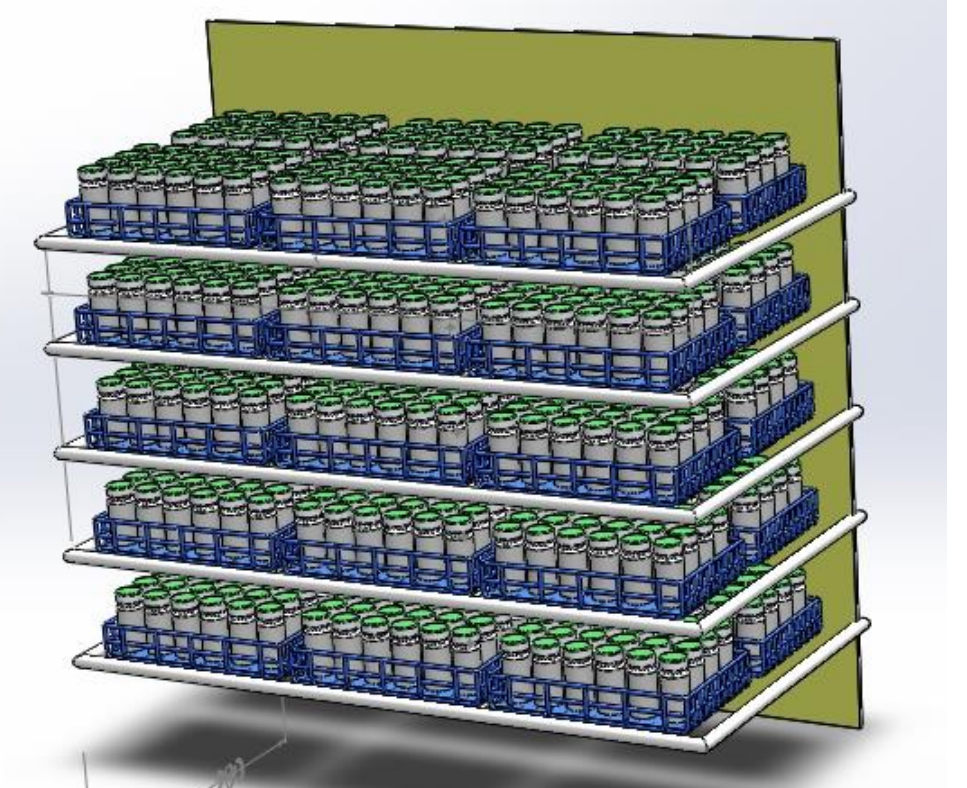
\includegraphics[width=0.5\linewidth]{figures/4-lateralcharolas2}
	\caption{Vistas laterales de la insulina acomodada dentro de la cámara.}
		Fuente: Elaboración propia usando \texttt{SolidWorks.}
	\label{fig:4-lateralcharolas1}
\end{figure}
 

En la figura  \ref{fig:4-superiorlcharolas}, vemos otra vista del arreglo de las charolas dentro de la cámara de refrigeración.

\begin{figure}[H]
	\centering
	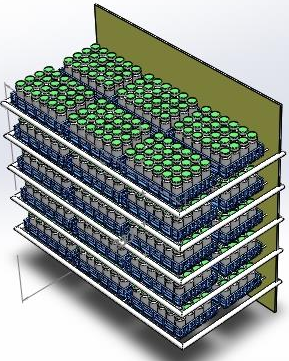
\includegraphics[width=0.5\linewidth]{figures/4-superiorlcharolas}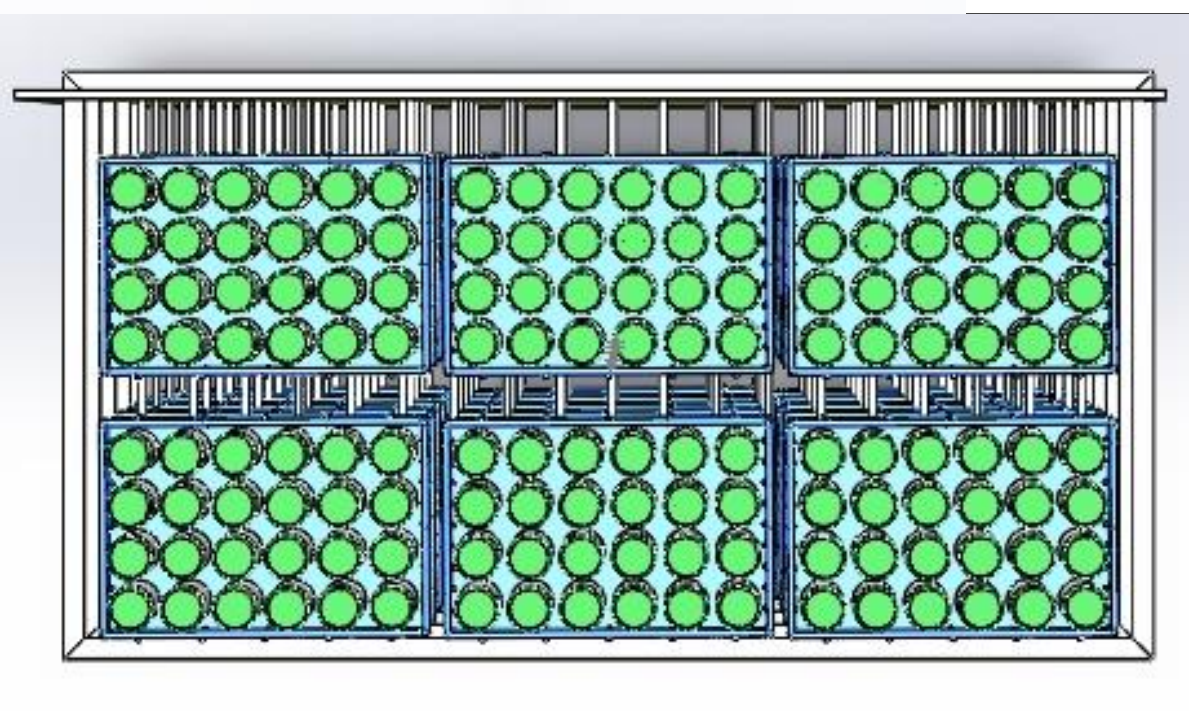
\includegraphics[width=0.6\linewidth]{figures/4-superiorlcharolas2}
	\caption{Vista superior de la cámara de refrigeración llena.}
		Fuente: Elaboración propia usando \texttt{SolidWorks.}
	\label{fig:4-superiorlcharolas}
\end{figure}

 



\subsection{Tipo de aislamiento térmico}

Algunos de los factores clave a considerar en la selección del aislamiento térmico incluyen su frecuencia de uso, área de aplicación, costo, eficiencia y el espacio que ocupará. Dado estos parámetros, el poliuretano expandido se presenta como una opción ideal, ya que cumple con los requisitos mencionados de manera eficiente. En la tabla \ref{tabla:aislantes} se presenta un resumen comparativo de los datos de diversos aislantes térmicos disponibles en el mercado.\\
El frigerante a utilizar para la conservación de insulina dentro de la cámara de refrigeración, una opción recomendada será el  \textbf{R-142b} o \textbf{R-600a}. Ambos refrigerantes son eficientes, seguros y adecuados para sistemas de refrigeración médica que requieren un control preciso de la temperatura. El R-600a es una opción más ecológica, ya que tiene un bajo impacto ambiental y no daña la capa de ozono, mientras que el R-142b es comúnmente utilizado en aplicaciones médicas por su estabilidad y rendimiento.

\begin{table}[H]
	\centering
	\caption{Conductividad térmica del aislamiento de cámaras frigoríficas}Fuente Fuente: Extraído del manual de Fundamentos (AHSRAE,1967).
	\begin{tabular}{lc}
		\hline
		\textbf{Aislamiento} & \textbf{Conductividad térmica ($k,\; Btu\; in/h ft °F)$} \\
		 \hline
		Tablero de poliuretano (R-11 expandido)   & 0.16 a 0.18 \\  
		Polisocianurato celular (R-141b expandido) & 0.19 \\  
		Poliestireno extruido (R-142b)             & 0.24 \\  
		Poliestireno expandido (R-142b)            & 0.26 \\  
		Tablero de corcho                          & 0.30 \\  
		Vidrio espumado                            & 0.31 \\ 
		\hline 
	\end{tabular}
	\label{tabla:aislantes}
\end{table}



\section{Balances de carga térmica}
Tomando como referencia las tablas de datos mostrados en las tablas, \ref{tabla:condsinsulina} y \ref{tabla:aislantes} calcularemos la carga térmica total que estará abatiendo la cámara frigorífica.

\subsection{Condiciones exteriores de diseño:}  
 \begin{equation} 
 \begin{aligned}
 	 T_{BS} &= 25^\circ C [77^\circ F] \\
 	T_{BH} &= 20^\circ C [68^\circ F] \\
 	H_R &= 90\%\\
 	T_{alamacenamiento}& = T_{alm} = 3^\circ C [37.4\degree F]
 	 \end{aligned} 		 
 \end{equation}
 
	
 \subsection{Aislamiento térmico: Poliuretano expandido}
	Tomando en consideración la aplicación del poliuretano expandido, que es el principal aislante térmico en consideración la refrigeración de productos médicos, 
	
 \begin{equation}
 	 \begin{aligned}
 	 k &= 0.16\frac{BTU \cdot pulg}{ft^2 \cdot hr \cdot ^\circ F}\\
 	 e&=\Big(\frac{1}{5}\Big)\Delta T = \Big(\frac{1}{5}\Big)\big(T_{BS}- T_{alm}\big)\\ 	
 	 &=  \Big(\frac{1}{5}\Big)\times (25-3)^\circ =4{.}4 cm\\
 	 &= 4{.}4 cm \times \dfrac{1\; in}{2{.}54 cm} =1{.}732283\; in\\
 	 \therefore e&= 1{.}74\; in \text{, para cálculo máximo}
 \end{aligned}
 \end{equation}
 \subsection{Coeficiente de película}
	Este coeficiente de película es considerado con el manual de ASHRAE, gracias a los
	estudios cualitativos del comportamiento de los factores de calor por convección en
	condiciones promedio.	
	\begin{equation}
		\begin{aligned}
			h_i &= 1.6 \, \frac{{BTU}}{{pie}^2 \cdot {hr} \cdot \degree F} \\
			h_e &= 6\, \frac{{BTU} \cdot {pulg}}{{pie}^2 \cdot {hr} \cdot \degree F}
		\end{aligned}
	\end{equation}
	
 \subsubsection{Coeficiente de transferencia de calor}
Para las áreas de las paredes de la cámara frigorífica, se propone una tabla específica
las áreas largas, cortas, piso y techo, observe la figura \ref{fig:paredes-peliculas} para detalles de la ecuación.

  \begin{equation}
  	\begin{aligned}
  		U &= \frac{1}{\frac{1}{f_i} + \frac{e_{\text{lamina}}}{k_{\text{lamina}}} + \frac{e_{\text{poliuretano}}}{k_{\text{poliuretano}}} + \frac{e_{\text{lamina}}}{k_{\text{lamina}}} + \frac{1}{f_e}} \\
  		U &= \frac{1}{\frac{1}{f_i} + \frac{2 e_{\text{lamina}}}{k_{\text{lamina}}} + \frac{e_{\text{poliuretano}}}{k_{\text{poliuretano}}} + \frac{1}{f_e}} \\
  	\end{aligned}
  	\label{eq:coef-transf-calor}
  \end{equation}


\begin{figure}[H]
	\centering
	\begin{tikzpicture}	
		% Dibujar las capas de la pared
		% Capa de Poliuretano
		\fill[pattern=north east lines, pattern color=teal] (-1,0) rectangle (1,6);
	
				\node at (0,6.3) {\textbf{\textcolor{teal}{Poliuretano}}};
		
		% Láminas Pintro exteriores
		\draw[thick, gray] (-2,0) -- (-2,6);
		\draw[thick, gray] (2,0) -- (2,6);
		
		\node[gray] at (-2,-0.3) {\textbf{Lámina Pintro}};
		\node[gray] at (2,-0.3) {\textbf{Lámina Pintro}};
		
		% Coeficiente de Película interior (fi)
		\draw[blue, thick, <->] (-3,0) -- (-3,6);
		\node[blue, rotate=90] at (-3.8,3) {$f_i$ \textbf{Coeficiente}};
		\node[blue, rotate=90] at (-3.4,3) {\textbf{de Película}};
		
		% Coeficiente de Película exterior (fe)
		\draw[blue, thick, <->] (3,0) -- (3,6);
		\node[blue, rotate=90] at (3.4,3) {$f_e$ \textbf{Coeficiente}};
		\node[blue, rotate=90] at (3.8,3) {\textbf{de Película}};	
	\end{tikzpicture}
	\caption{Pared Compuesta propuesta para la cámara frigorífica} Fuente: Elaboración propia usando \LaTeX \; y \texttt{Tikz}
	\label{fig:paredes-peliculas}
\end{figure}
 
\subsection{Cálculo térmico de las paredes}
\subsubsection{Cálculo de áreas}
Se hará el cálculo de las áreas superficiales de cada elemento que mantiene almacenado
el producto a transportar, tomando por supuesto las áreas superficiales exteriores como
el punto de partida de dicho calculo.
\begin{equation}
	\begin{aligned}
		\text{Norte:}\quad A_n &=l\times  h=  0.6\, m \times 0.512\, m = 0.3072\, m^2 \times \frac{10.76\, ft^2}{1\, m^2} = 3.299\, ft^2 \\ 
		\text{Sur:}\quad A_s &=l\times h=  0.6\, m \times 0.512\, m = 0.3072\, m^2 \times \frac{10.76\, ft^2}{1\, m^2} = 3.299\, ft^2 \\ 
		\text{Oriente:} \quad A_o &=l\times h= 0.6\, m \times 0.6\, m = 0.36\, m^2 \times \frac{10.76\, ft^2}{1\, m^2} = 3.867\, ft^2 \\ 
		\text{Poniente:}\quad A_p &=l\times h= 0.6\, m \times 0.6\, m = 0.36\, m^2 \times \frac{10.76\, ft^2}{1\, m^2} = 3.867\, ft^2 \\ 
		\text{Piso y Techo:}\quad A_{pt} &=l\times h=  0.6\, m \times 0.6\, m = 0.36\, m^2 \times \frac{10.76\, ft^2}{1\, m^2} = 3.867\, ft^2
	\end{aligned}
	\label{eq:area-paredes}
\end{equation}

\textbf{Nota:}  Abatir carga térmica en un periodo de 22 horas, este parámetro fue seleccionado por
dos razones en el planteamiento del problema, primero, el producto llega a temperatura "ideal" de distribuidor, así que no
se retirará carga térmica de calor latente, entonces, la capacidad o riesgo de falla, es casi
nula, y por último el segundo factor, fue tomar en consideración que entre más rápido se
necesite abatir una carga térmica, más grande tendrá que ser el dispositivo.

\subsubsection{Transmisión de calor en paredes, pisos y techo}

Para este cálculo es necesario consultar la ecuación \ref{eq:coef-transf-calor} el cual nos indica un coeficiente
a considerar con los parámetros tanto de calor por convección, y el factor del aislante térmico.

\begin{equation}
	U = 
	\frac{1}{\left( \frac{1}{1.6} \right) + \left( \frac{2\times 0.017 }{30.04} \right)+\left( \frac{1.74}{0.17}\right) + \left( \frac{1}{6}\right)} 
	= 0.0808 \, \frac{ {BTU}}{ {ft}^2 \cdot  {hr} \cdot \degree F}
	\label{eq:u}
\end{equation}

De manera que en la figura \ref{fig:paredes-peliculas2} se resumen los valores de los coeficientes de transferencia. 

\begin{figure}[H]
	\centering
	\begin{tikzpicture}	
		% Dibujar las capas de la pared
		% Capa de Poliuretano
		\fill[pattern=north east lines, pattern color=teal] (-1,0) rectangle (1,6);
		
		\node at (0,7) {\textbf{\textcolor{teal}{Poliuretano}}};
		
		% Láminas Pintro exteriores
		\draw[thick, gray] (-2,0) -- (-2,6);
		\draw[thick, gray] (2,0) -- (2,6);
		
		\node[gray] at (-2,-0.3) {{\small \textbf{Lámina Pintro Cal 26}}};
		\node[gray] at (2,-0.3) {{\small  \textbf{Lámina Pintro Cal 26}}};
		
		% Coeficiente de Película interior (fi)
		\draw[blue, thick, <->] (-3,0) -- (-3,6);
		\node[blue, rotate=90] at (-4,3) {$f_i = 1.6 \frac{ {Btu}}{h \cdot ft^2 \cdot \degree F}$};
		\node[blue, rotate=90] at (-3.4,3) {\textbf{Coeficiente de Película}};
		
		% Coeficiente de Película exterior (fe)
		\draw[blue, thick, <->] (3,0) -- (3,6);
		\node[blue, rotate=90] at (3.4,3) {$f_e = 6 \frac{ {Btu}}{h \cdot ft^2 \cdot \degree F}$};
		\node[blue, rotate=90] at (4,3) {\textbf{Coeficiente de Película}};	
		
		% Coeficiente de Conductividad (k) para Poliuretano
		\node[red] at (0,6.3)  {$k = 0.17 \frac{ {Btu} \cdot in}{h \cdot ft^2 \cdot \degree F}$};
		
		% Coeficiente de Conductividad (k) para Pintro
		\node[red] at (0,-1) {$k = 30.04 \frac{ {Btu} \cdot in}{h \cdot ft^2 \cdot \degree F}$};
	\end{tikzpicture}
	\caption{Pared Compuesta propuesta para la cámara frigorífica} Fuente: Elaboración propia usando \LaTeX \; y \texttt{Tikz}
	\label{fig:paredes-peliculas2}
\end{figure}


\subsubsection{Carga térmica por paredes}
La carga térmica para cada muro de la cámara de refrigeración se calcula usando la fórmula:

\begin{equation} 
	Q = A \cdot U \cdot \Delta T
	\label{eq:carga-termica}
\end{equation}
Definimos las diferencias de temperatura
\begin{equation}
	\begin{aligned}		 
		 \Delta T_n & = T_{bs} - t_{almac} = 77 - 37.4 = 39.6 \,  \degree F \\  
		 \Delta T_s & = T_{bs} - t_{almac} + t_{almac} = 77 - 37.4 + 37.4 = 77 \,  \degree F \\  
		 \Delta T_o & = T_{bs} - t_{almac} + t_{almac} = 77 - 37.4 + 37.4 = 77 \,  \degree F \\  
		 \Delta T_p & = T_{bs} - t_{almac} + t_{almac} = 77 - 37.4 + 37.4 = 77 \,  \degree F \\  
		 \Delta T_{piso} & = T_{bs} + 9 + t_{almac} = 77 + 9 + 37.4 = 123.4 \, \degree F
	\end{aligned}
	\label{eq:dif-temp-paredes}
\end{equation}

 
Ahora reemplazando los resultados de \ref{eq:area-paredes}, \ref{eq:u}  y \ref{eq:dif-temp-paredes} en la ecuación \ref{eq:carga-termica} obtendremos la carga térmica para cada pared de nuestra cámara de refrigeración.
  
\begin{equation}
	\begin{aligned}
		\text{Norte:}&\\ 
		Q_n &= A_n \cdot U \cdot \Delta T_n = 3.299 \, {ft}^2 \cdot 0.0808 \, \frac{{{BTU}}}{{{ft}^2 \cdot \degree F}} \cdot (39.6 \degree F) \\
		& = 3.299 \times 0.0808 \times 39.6 \\
		& \approx 10.639\, {BTU/hr} \\ 
		\therefore Q_n &= 10.6 \, {BTU/hr} \\[1em]
		\text{Sur:}&\\
		Q_s &= A_s \cdot U \cdot \Delta T_s = 3.299 \, {ft}^2 \cdot 0.0808 \, \frac{{{BTU}}}{{{ft}^2 \cdot \degree F}} \cdot (77 - 37.4 + 37.4) \\
		& = 3.299 \times 0.0808 \times 77 \\
		& \approx 20.891\, {BTU/hr} \\ 
		\therefore Q_s &= 20.9 \, {BTU/hr} \\[1em]
		\text{Oriente:}&\\
		Q_o &= A_o \cdot U \cdot \Delta T_o = 3.867 \, {ft}^2 \cdot 0.0808 \, \frac{{{BTU}}}{{{ft}^2 \cdot \degree F}} \cdot (77 - 37.4 + 37.4) \\
		& = 3.867 \times 0.0808 \times 77 \\
		& \approx 23.144\, {BTU/hr} \\ 
		\therefore Q_o &= 23.1 \, {BTU/hr} \\[1em]
		\text{Poniente:}&\\
		Q_p &= A_p \cdot U \cdot \Delta T_p = 3.867 \, {ft}^2 \cdot 0.0808 \, \frac{{{BTU}}}{{{ft}^2 \cdot \degree F}} \cdot (77 - 37.4 + 37.4) \\
		& = 3.867 \times 0.0808 \times 77 \\
		& \approx 23.144\, {BTU/hr} \\ 
		\therefore Q_p &= 23.1 \, {BTU/hr} \\[1em]
		\text{Piso:}&\\
		Q_{piso} &= A_{pt} \cdot U \cdot \Delta T_{piso} = 3.867 \, {ft}^2 \cdot 0.0808 \, \frac{{{BTU}}}{{{ft}^2 \cdot \degree F}} \cdot (77 + 9 - 37.4) \\
		& = 3.867 \times 0.0808 \times 48.6 \\
		& \approx 15.160\, {BTU/hr} \\ 
		\therefore Q_{piso} &= 15.2 \, {BTU/hr}  =Q_{techo}
	\end{aligned}
\end{equation}


 \begin{equation}
Q_{T_{paredes}} = Q_n +Q_s + Q_o + Q_p + Q_{piso} +q_{techo} = 108.1  {BTU/hr}
 \end{equation}
 
 \subsubsection{Carga térmica del producto}
 Para calcular la carga térmica del producto, es fundamental considerar que no hay calor latente que remover en el proceso de almacenamiento. Sin embargo, existe un calor sensible que debe tenerse en cuenta. Almacenaremos la insulina a una temperatura específica, lo que nos permite calcular la carga térmica sensible considerando la tasa de transferencia de masa y el calor específico del producto.\\
 La tasa de flujo de masa se calcula de la siguiente manera: 
 \begin{equation}
 	\begin{aligned}
 		\dot{m} &= (F \cdot R) \cdot \left( \frac{2,200 \, \text{lb}}{1 \, \text{TM}} \right) \cdot \left( \frac{1 \, \text{día}}{24 \, \text{hrs}} \right) \\
 		\dot{m} &=1TM\left( \frac{2,200 \, \text{lb}}{1 \,TM  } \right) \cdot \left( \frac{1 \, \text{día}}{24 \, \text{hrs}} \right) \\
 		\dot{m} &= 91.6666 \, \frac{\text{lb}}{\text{hr}}
 	\end{aligned}
 \end{equation}
La carga térmica sensible de la insulina \( Q_{\text{insulina}} \) se obtiene con la fórmula:

\begin{equation}
	\begin{aligned}
		Q_{\text{insulina}} &= \dot{m} \cdot C_p \cdot (T_{\text{en}} - T_{\text{alm}}) \\
		C_p &= 0.35 \, \frac{ {BTU}}{ {lb} \cdot \degree F}
	\end{aligned}
\end{equation}

Sustituyendo los valores:

\begin{equation}
	\begin{aligned}
		Q_S &=  91.6666 \, \frac{ {lb}}{ {hr}}\times \left( 0.35 \, \frac{ {BTU}}{ {lb} \cdot \degree F} \right) \times ( 6 - 3)=192.5 {BTU/hr} \\
		\therefore Q_{insulina} &=192.5 {BTU/hr}
	\end{aligned}
\end{equation}

\subsubsection{Carga térmica por Infiltración}
En este apartado de los cálculos, es importante aclarar varios factores que influyen en la selección del sistema de refrigeración para la conservación de insulina. Uno de los primeros aspectos a considerar en un espacio refrigerado es cuantificar la cantidad de calor que puede infiltrarse en la cámara. Para realizar este análisis de manera precisa, se debe comenzar por calcular la capacidad volumétrica del área a refrigerar, lo cual implica determinar el volumen total del espacio. Este valor es fundamental para dimensionar adecuadamente el equipo de refrigeración necesario.

Además del volumen, se deben tener en cuenta otros factores importantes, como la ubicación geográfica, la carga térmica generada por las operaciones internas y las condiciones ambientales externas que puedan afectar el rendimiento del sistema. Estos datos son esenciales para diseñar un sistema eficiente que mantenga las condiciones óptimas de temperatura y humedad dentro de la cámara refrigerada. ASHRAE proporciona una tabulación de datos que indica la cantidad de cambios de aire por hora en función de la capacidad volumétrica del espacio, lo que permite calcular con precisión la carga térmica total del sistema. 
 
 \begin{equation}
 	\begin{aligned}
 		V&=l\times a\times h\\
 		&=0.6m \times 0.6m\times 0.51m\\
 		&=0.1836 m^3 \times \left(35.31 \frac{ft^3}{m^3}\right)\\
  \therefore V&= 6.483 ft^3 
 	\end{aligned}
 \end{equation}
 
 Usando la tabla \ref{tabla:4-promedio-aire24h}, para poder encontrar el factor que indica los cambios de aire por cada  24 horas, de ser necesario, interpolar entre los valores aproximados para una mayor  exactitud
 
 \begin{table}[H]
 	\centering
 	\caption{ Promedio de cambios de aire en 24 horas para cámaras de
 		almacenaje debido a la apertura de puertas e infiltración} Fuente: Extraído del manual de Fundamentos ASHRAE, (1981). \\
 		\label{tabla:4-promedio-aire24h}		
 	\begin{tabular}{cccccc}
 		\hline
 		& \multicolumn{2}{c}{Cambios de aire en 24 horas}                             &                                       & \multicolumn{2}{c}{Cambios de aire en 24 horas}                           \\ \cline{2-3} \cline{5-6} 
 		\multirow{-2}{*}{\begin{tabular}[c]{@{}c@{}}Volumen\\  $ft^3$\end{tabular}} & Arriba de 32°F                       & Abajo de 32°F                        & \multirow{-2}{*}{Volumen $ft^3$}         & Arriba de 32°F                      & Abajo de 32°F                       \\ \hline
 		{\color[HTML]{DA8292} \textbf{200}}                                      & {\color[HTML]{DA8292} \textbf{44.0}} & {\color[HTML]{DA8292} \textbf{33.5}} &  \textbf{6,000} &  \textbf{6.5} & \textbf{5.0} \\
 		300                                                                      & 34,5                                 & 26.2                                 & 8.000                                 & 5.5                                 & 4.3                                 \\
 		400                                                                      & 29,5                                 & 22.5                                 & 10,000                                & 4.9                                 & 3.8                                 \\
 		500                                                                      & 26.0                                 & 20.0                                 & 15.000                                & 3.9                                 & 3.0                                 \\
 		600                                                                      & 23,0                                 & 18.0                                 & 20,000                                & 3.5                                 & 2.6                                 \\
 		800                                                                      & 20.0                                 & 15.3                                 & 25,000                                & 3.0                                 & 2.3                                 \\
 		1 ,000                                                                   & 17.5                                 & 13.5                                 & 30,000                                & 2.7                                 & 2.1                                 \\
 		1 ,500                                                                   & 14.0                                 & 11.0                                 & 40,000                                & 2.3                                 & 1.8                                 \\
 		2,000                                                                    & 12.0                                 & 9.3                                  & 50,000                                & 2.0                                 & 1.6                                 \\
 		3,000                                                                    & 9.2                                  & 7.4                                  & 75,000                                & 1.6                                 & 1.3                                 \\
 		4,000                                                                    & 8.2                                  & 6.3                                  & 100,000                               & 1.4                                 & 1.1                                 \\
 		6,000                                                                    & 7.2                                  & 5.6                                  &                                       &                                     &                                     \\ \hline
 	\end{tabular}
 	\end{table}
 	
 	
 	Para poder obtener factor del calor removido en el aire es necesario tener como dato la
 	temperatura de bulbo seco y la temperatura de almacenaje, así apoyándose de la tabla \ref{tabla:4-calor-removido} encontrar el factor de calor removido.
 
 	\begin{table}[H]
 		\centering
 		\caption{Calor removido en aire de enfriamiento en las condiciones de almacenamiento (BTU por pie cúbico)} 
 		Fuente: Extraído del manual de Fundamentos ASHRAE 1981.
 		\label{tabla:4-calor-removido}
 		\begin{tabular}{ccccccccc}
 			\hline
 			& \multicolumn{8}{c}{Temperatura del aire exterior °F}                                                                    \\ \cline{2-9} 
 			& \multicolumn{2}{c}{85}                      & \multicolumn{2}{c}{90} & \multicolumn{2}{c}{95} & \multicolumn{2}{c}{100} \\ \cline{2-9} 
 			& \multicolumn{8}{c}{Porciento de Humedad Relativa}                                                                       \\ \cline{2-9} 
 			\multirow{-4}{*}{\begin{tabular}[c]{@{}c@{}}Temperatura de\\ la cámara de\\ Almacenamiento\\ °F\end{tabular}} & 60   & 60                                   & 70         & 80        & 50         & 60        & 50         & 60         \\ \hline
 			25                                                                                                            & 0.39 & 0.43                                 & 0.69       & 0.91      & 0.93       & 1.20      & 2.54       & 1.51       \\
 			20                                                                                                            & 0.62 & 0.56                                 & 0.89       & 1.12      & 1.14       & I.41      & 2.68       & 1.71       \\
 			15                                                                                                            & 0.65 & 0.69                                 & 1.08       & 1.31      & 1.33       & 1.60      & 2.80       & 1.91       \\
 			10                                                                                                            & 0.77 & 0.82                                 & 1.26       & 149       & 1.51       & 1.78      & 2.93       & 2.09       \\
 			{\color[HTML]{DA8292} \textbf{5}}                                                                             & 0.89 & {\color[HTML]{DA8292} \textbf{0.94}} & 1.43       & 1.66      & 1.68       & 1.94      & 3.05       & 2.25       \\
 			{\color[HTML]{DA8292} \textbf{0}}                                                                             & 1.01 & {\color[HTML]{DA8292} \textbf{1.05}} & 1.59       & 1.81      & 1.83       & 2.10      & 3.16       & 2.41       \\
 			-5                                                                                                            & 1.13 & 1.17                                 & 1.74       & 1.96      & 1.99       & 2.25      & 3.28       & 2.56       \\
 			-10                                                                                                           & 1.24 & 1.29                                 & 1.88       & 2.10      & 2.13       & 2.39      & 3.40       & 2.70       \\ \hline
 		\end{tabular}
 	\end{table}
 	
 	
 	
 	\begin{equation}
 		\begin{aligned}
 			Q_{\text{Infiltración}} &= (V) \cdot \left( \frac{\text{Cambios}}{24 \, \text{hrs}} \right) \cdot (\text{Calor removido}) \cdot f \\
 			Q_{\text{Infiltración}} &= (6.483 {ft}^3) \cdot \left( 33.5 \, \frac{\text{Cambios}}{24 \, \text{hrs}} \right) \cdot \left(0.90  \, \frac{{BTU}}{{ft}^3} \right) \cdot 0.6 \\
 			Q_{\text{Infiltración}} &=117.27747\, \frac{{BTU}}{{hr}}
 		\end{aligned}
 	\end{equation}
 	
 	
 	
 	\subsubsection{Carga del Motor eléctrico}
 	
 	Este cálculo se basa en la preselección del equipo adecuado. Al hablar de un dispositivo diseñado para refrigerar insulina, es fundamental considerar el uso del Thermo King y sus componentes. El evaporador, que se instala dentro de la cámara refrigerada, se toma en cuenta dentro de los cálculos de carga térmica.\\
 	Para realizar el cálculo de la carga térmica es necesario disponer de los datos del motor y la cantidad de equipo dentro de la cámara. Para determinar el calor emitido por estos dispositivos, es necesario consultar la tabla \ref{tabla:4-motores-calor}, que contiene la información requerida para su aplicación en el área refrigerada.
 	
 	
 	
 	\begin{table}[H]
 		\centering
 		\caption{alor disipado por los motores eléctricos}
 		Fuente: Extraído del manual de Fundamentos ASHRAE 1981
 		 \label{tabla:4-motores-calor}
 		\begin{tabular}{cccc}
 			\hline
 			\multicolumn{1}{c|}{}                                                                         & \multicolumn{3}{c}{\textit{BTU por (hp)/(hora)}}                                                                                                                                                                                       \\ \cline{2-4} 
 			\multicolumn{1}{c|}{\multirow{-2}{*}{\begin{tabular}[c]{@{}c@{}}HP\\ del motor\end{tabular}}} & \begin{tabular}[c]{@{}c@{}}Motor y ventilador\\ dentro del cuarto\end{tabular} & \begin{tabular}[c]{@{}c@{}}Motor fuera y\\ ventilador dentro\end{tabular} & \begin{tabular}[c]{@{}c@{}}Motor dentro y\\ ventilador fuera\end{tabular} \\ \hline
 			1/8 a 1/2                                                                                     & 4250                                                                           & 2.545                                                                     & 1,700                                                                     \\
 			{\color[HTML]{DA8292} \textbf{1/2 a 3}}                                                       & {\color[HTML]{DA8292} \textbf{3,700}}                                          & 2,545                                                                     & 1,150                                                                     \\
 			3 a 20                                                                                        & 2,950                                                                          & 2,545                                                                     & 400                                                                       \\ \hline
 		\end{tabular}
 	\end{table}
 	Tomando como apoyo la ecuación del calor en motores y sustituyendo las variables a considerar de la tabla \ref{tabla:4-motores-calor} se obtiene el calor generado por la cantidad de motores
 	\begin{equation}
 		\begin{aligned}
 			Q_{\text{Motores}} &= (\#\text{Motores}) (\text{HP}) (\text{Calor disipado por los motores}) \\
 			Q_{\text{Motores}} &= (1)(1.20 \,  {HP}) \left( 2545 \, \frac{ {BTU}}{ {hr} \cdot  {HP}} \right) \\
 			Q_{\text{Motores}} &= 3054 \, \frac{ {BTU}}{ {hr}} 
 		\end{aligned}
 	\end{equation}
 	\subsubsection{Carga por iluminación}
 	Se toma en consideración la carga térmica promedio generada en una situación crítica
 	donde se toma 1 watt por cada pie cuadrado, y el total del área superficial total del techo.
 	
 	\begin{equation}
 		\begin{aligned}
 			Q_{iluminacion} &= (\text{Largo}_{Ext})(\text{Ancho}_{Ext})(\text{Factor de conversión})(\text{Dato de Norma})(\text{FC}_{Norma}) \\
 			&= 0.6\, m \times 0.6\, m \times 10.76\, \frac{ft^2}{m^2} \times 1\, \frac{Watt}{ft^2} \times 3.41\, \frac{BTU}{hr \cdot Watt} \\
 		\therefore Q_{iluminacion} &=  13.208 \frac{BTU}{hr}
 		\end{aligned}
 	\end{equation}
 	 \subsection{Carga térmica total}
 	
 	 \begin{equation}
 	 	\begin{aligned}
 	 		Q_{subtotal} &=Q_{T_paredes}+Q_{insulina}+Q_{Infiltracion}+ Q_{motores}+ Q_{iluminacion} \\
 	 		&= (108.1+192.5+ 117.3 + 3054+13.208)BTU/hr\\
 	 		 \therefore Q_{subtotal} &=3,485.108 BTU/hr
 	 	\end{aligned}
 	 \end{equation}
 	Considerando un factor de seguridad por cuestiones de variaciones de temperatura originadas
 	por los cambios climáticos sufridos por el país, que no son consideradas dentro de los
 	parámetros calculados.
 	 \begin{equation}
 		\begin{aligned}
 			10\% \; F.S &=34.851 Btu/h\\
 			\therefore Q_{Total} &=3,519.951 BTU/hr
 		\end{aligned}
 	\end{equation}
 	
 \section{Selección de equipo}	

 
 \subsection{Unidad condensadora}
 
 En esta sección, es fundamental contar con una amplia variedad de catálogos de unidades condensadoras tipo Thermo King para realizar una selección eficiente del equipo adecuado. La selección de la unidad condensadora Thermo King incluye los componentes esenciales del proceso de refrigeración, como la unidad evaporadora, la unidad de expansión, el condensador o intercambiador de calor, y el compresor. Con estos elementos incluidos en el sistema Thermo King, solo queda seleccionar con base en los parámetros de temperatura de almacenamiento y la carga térmica con la que operará la unidad condensadora.
 
 De acuerdo con el Catálogo Thermo King, categoría Advancer A-500 (\hyperref[fig:axo-manual-thermo-king]{anexo 7}) ), la capacidad de la unidad condensadora a una temperatura de operación de $-20^\circ C$ (muy cercana a los $-18^\circ C$ calculados) es de 
 \[
 10,400\, W \left( 35,464\, \frac{BTU}{hr} \right)
 \]
 Comparando con los cálculos obtenidos de 
 \[
	3,485.108 \, \frac{BTU}{hr}
 \]
 hay una diferencia aproximada de 
 \[
 1,000\, \frac{BTU}{hr}
 \]
 lo que representa una variación del 2.78\%. Esta pequeña diferencia confirma que la selección del equipo es adecuada. Para más detalles, consulte el catálogo completo en el \hyperref[fig:axo-manual-thermo-king]{anexo 7}.
 
 \begin{figure}[H]
 	\centering
 	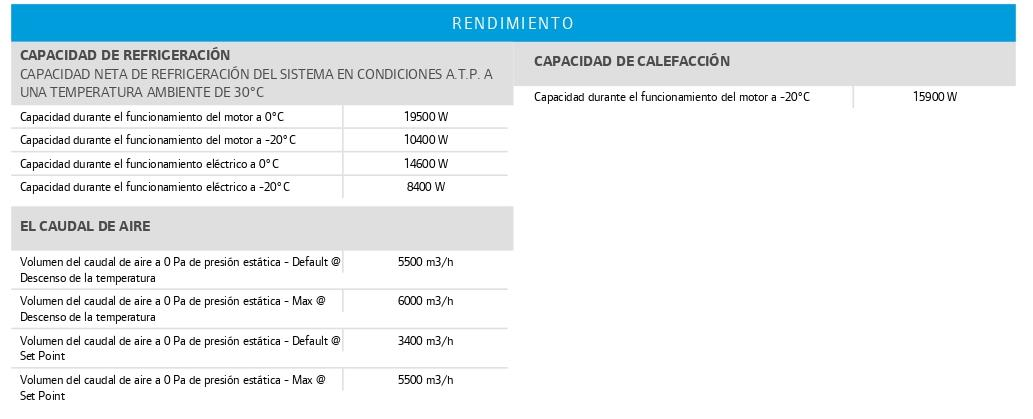
\includegraphics[width=0.8\linewidth]{figures/4-seleccion-condensador}
 	\caption{Tabla de datos recortado del catálogo de especificaciones Thermo King del anexo 7.}
 	Fuente: \hyperref[fig:axo-manual-thermo-king]{(Thermo King, 2024)}
 	\label{fig:4-seleccion-condensador}
 \end{figure}
 
 \section{Diseño del sistema eléctrico}
 Es fundamental implementar un sistema eléctrico seguro (ver figura \ref{fig:4-frontalcharolas}) para una cámara de refrigeración destinada al almacenamiento de insulina, dada la importancia de mantener condiciones óptimas para la conservación de productos farmacéuticos. Un sistema eléctrico confiable garantiza que la temperatura dentro de la cámara se mantenga constante y segura, evitando la degradación del fármaco y asegurando su efectividad. En la figura \ref{fig:4-diag-electrico} se puede apreciar un acercamiento al diagrama resumido que se propone, para más detalles vea el \hyperref[axo:diag-electrico]{anexo 3}. \\
 Prevención de Incendios: Un diseño eléctrico defectuoso o inadecuado puede provocar cortocircuitos o sobrecargas eléctricas, lo que incrementa significativamente el riesgo de incendios. Esto no solo puede causar daños al equipo, sino que también compromete la seguridad de las instalaciones y del personal.\\
  \textbf{Mantenimiento del Equipo}: Un sistema eléctrico bien diseñado contribuye al funcionamiento óptimo y prolongado de los equipos de refrigeración. Esto reduce la probabilidad de fallas y preserva los componentes en buen estado por más tiempo, lo cual es crucial en un entorno donde la integridad de los productos farmacéuticos es prioritaria.\\
\textbf{Cumplimiento Normativo}: En el ámbito farmacéutico, existen regulaciones y estándares específicos que deben cumplirse para el almacenamiento de productos sensibles como la insulina. Asegurarse de cumplir con estos requisitos es esencial para evitar multas y sanciones, además de garantizar la seguridad y eficacia de los productos almacenados.


\subsection{Esquema a bloques del funcionamiento del sistema eléctrico.}

El esquema de la figura \ref{fig:4-blockelectric} incluye las siguientes protecciones para mantener seguros y protegidos los componentes del sistema de refrigeración:
\begin{itemize}

	\item[$\odot$] Interruptor de Circuito: Permite cortar el suministro eléctrico en caso de sobrecarga o cortocircuito, protegiendo así los componentes eléctricos.

	\item[$\odot$] Protección Contra Sobrecorriente: Previene daños al sistema eléctrico en caso de corrientes excesivas.

\item[$\odot$] Protección Contra Sobretensión: Salvaguarda al sistema contra picos de voltaje que podrían dañar los componentes eléctricos.

\item[$\odot$] Controlador de Temperatura: Asegura que la temperatura dentro de la cámara de refrigeración se mantenga dentro de los límites seguros.

\item[$\odot$] Sensor de Temperatura y Humedad: Monitorea continuamente las condiciones de la cámara, garantizando el correcto funcionamiento del sistema de refrigeración.

\end{itemize}
 \begin{figure}[H]
	\centering 
	\begin{tikzpicture}[node distance=2cm and 1cm]
		
		% Bloques del sistema
		\node (input) [block] {Entrada de energía};
		\node (switch) [block, right=of input] {Interruptor de circuito};
		\node (protector) [block, right=of switch] {Protección contra sobrecorriente};
		
		% Filtro de secado más abajo
		\node (controltemp) [block, below=of protector] {Control de temperatura};
		\node (compresor) [block, left=of controltemp] {Compresor y sistema de refrigeración};
		\node (evaporator) [block, left=of evaporator] {Evaporador};
		
		% un salto más
		\node (sobretension) [block, below=of evaporator] {Protección contra sobretensión};
		\node (sensor) [block, right=of sobretension] {Sensor de temperatura y humedad};
		\node (output) [block, right=of sensor] {Salida de energía};
		
		% Flechas entre los bloques
		\draw [arrow] (input) -- (switch);
		\draw [arrow] (switch) -- (protector);
		
		% Flecha hacia abajo
		\draw [arrow] (protector) -- (controltemp);
		
		% Flecha de vuelta a la izquierda
		\draw [arrow] (controltemp) -- (compresor);
		\draw [arrow] (compresor) -- (evaporator);
		
		\draw [arrow] (evaporator) -- (sobretension);
			\draw [arrow] (sobretension) -- (sensor);
			\draw [arrow] (sensor) -- (output);
		
	\end{tikzpicture}
	\caption{Esquema a bloques del sistema eléctrico.}
	Fuente: Elaboración propia usando \texttt{Tikz}
	\label{fig:4-blockelectric}
\end{figure} 



 \subsection{Protección contra sobrecarga}
 La protección contra sobrecarga es un mecanismo diseñado para evitar daños en un circuito eléctrico debido a corrientes excesivas. Este sistema se implementa para garantizar la seguridad del sistema eléctrico y proteger sus componentes de posibles fallas o daños. Es esencial contar con un dispositivo de protección contra sobrecarga en el sistema de refrigeración para asegurar su seguridad, fiabilidad y cumplimiento normativo.
 
 En el contexto del sistema de la cámara de refrigeración para este proyecto, se utilizará un disyuntor (ver figura \ref{fig:4-disyuntor}). Este dispositivo abrirá el circuito en caso de sobrecarga, y tras corregir cualquier fallo que se presente en el sistema, se podrá reiniciar manualmente, restableciendo así su funcionalidad original.
 
 \begin{figure}[H]
 	\centering
 	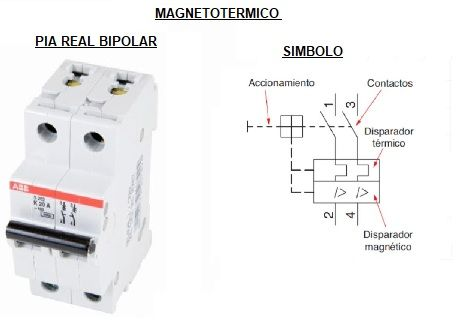
\includegraphics[width=0.6\linewidth]{figures/4-disyuntor}
 	\caption{Disyuntor simbología}
 	Fuente: \cite{areatecnologia}
 	\label{fig:4-disyuntor}
 \end{figure}
 	 
 \subsection{Protección Contra Cortocircuito}
 
 Un cortocircuito ocurre cuando se forma una conexión eléctrica no deseada entre dos puntos de un circuito que normalmente no deberían estar conectados. Esto puede resultar en corrientes extremadamente altas que fluyen a través del circuito, provocando sobrecalentamiento, incendios e incluso explosiones. Para proteger el sistema contra cortocircuitos, se implementará un fusible (ver figura \ref{fig:4-fusible}) que se colocará en serie en la conexión principal. Al detectar una corriente muy alta, el fusible se fundirá, impidiendo el paso de electricidad y protegiendo así la integridad de los componentes. Una vez corregido el fallo, el fusible puede ser fácilmente reemplazado por otro de características similares, permitiendo que el sistema vuelva a funcionar con normalidad.
 
 \begin{figure}[H]
 	\centering
 	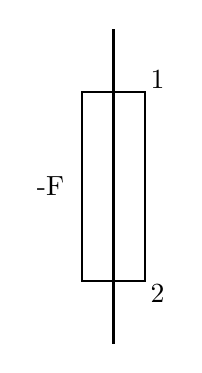
\begin{tikzpicture}[scale=0.8]
 		
 		% Draw the fuse body
 		\draw[thick] (0,0) rectangle (1,3); % Rectángulo del fusible
 		
 		% Draw the vertical line in the middle
 		\draw[thick] (0.5, -1) -- (0.5, 4); % Línea vertical del fusible
 		
 		% Draw the labels
 		\node at (-0.5, 1.5) {-F};
 		\node at (1.2, 3.2) {1}; % Punto 1 arriba
 		\node at (1.2, -0.2) {2}; % Punto 2 abajo
 		
 	\end{tikzpicture}
 	\caption{Simbología de un fusible}
 	Fuente: Elaboración propia usando \LaTeX y \texttt{Tikz}
 	\label{fig:4-fusible}
 \end{figure}
 
 
 \subsection{Diseño del Sistema de Seguridad Eléctrico}
 
 El diseño del sistema eléctrico es un aspecto crucial en la planificación y ejecución de cualquier instalación eléctrica. Garantizar la seguridad de las personas, proteger los productos farmacéuticos y prevenir incidentes son objetivos prioritarios en este proceso.
 
 \subsubsection{Metas de la segurida eléctrica}
 \begin{enumerate}
 	\item Salvaguardar la integridad física de las personas que interactúan con el sistema de refrigeración.
 	\item Proteger los equipos y componentes eléctricos de daños causados por condiciones anormales de operación.
 	\item Minimizar el riesgo de incendios y otros accidentes eléctricos.
 	\item Cumplir con las normativas y estándares de seguridad eléctrica aplicables.
 \end{enumerate}
 
 \subsubsection{Elementos del Sistema de Seguridad}
 \begin{itemize}
 	\item \textbf{Protección Contra Sobrecarga:} Se implementará un disyuntor que será el encargado de proteger el sistema (ver figura \ref{fig:4-disyuntor}).
 	\item \textbf{Protección Contra Cortocircuito:} Se instalará un fusible que impedirá el paso de corriente en caso de cortocircuito, protegiendo así los componentes del sistema.
 	\item \textbf{Sistemas de Puesta a Tierra:} Estos sistemas servirán para proteger a las personas de descargas eléctricas; el disyuntor también cumplirá esta función.
 	\item \textbf{Aislamiento Eléctrico:} Se utilizarán materiales y técnicas adecuadas para garantizar un aislamiento seguro de conductores y equipos, evitando descargas y arcos eléctricos.
 \end{itemize}
 
 Considerando todos estos puntos, se diseñará un circuito que sea seguro para el operador de la cámara y mantenga la continuidad operativa de las instalaciones eléctricas.  
 
 
 
 
 \subsection{Tablero de Control}
 
 El panel de control del equipo seleccionado cuenta con un Controlador SR-4 desarrollado por Thermo King, que incorpora los últimos avances tecnológicos. Este panel no solo supervisa y regula la temperatura, sino que también gestiona integralmente el funcionamiento de la unidad de manera eficiente. A través de una interfaz de máquina humana (HMI), el microprocesador en la caja de control proporciona una operación intuitiva y amigable para el operador, mostrando información de funcionamiento de manera rápida y precisa.
 
 La caja de control está estratégicamente ubicada en la puerta de servicio inferior para facilitar el acceso y el mantenimiento. Además, los puertos USB integrados permiten la recuperación sencilla de datos del sistema de registro, lo que proporciona una herramienta invaluable para el análisis y la optimización del rendimiento del equipo. Este diseño avanzado del panel de control no solo mejora la eficiencia operativa, sino que también garantiza un monitoreo detallado y una gestión efectiva de todas las funciones críticas del sistema de refrigeración.
 
 En la figura 3.13 se muestra el tablero de control del equipo seleccionado, junto con las funciones que permite acceder cada botón, destacando su amigabilidad para el operador.

\begin{figure}[H]
	\centering
 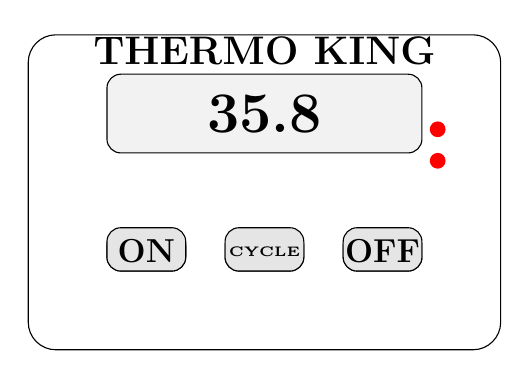
\begin{tikzpicture}
	% Draw the main panel
	\draw[rounded corners=10pt, fill=white] (0,0) rectangle (6,4);
	
	% Draw the screen
	\draw[rounded corners=5pt, fill=gray!10] (1,2.5) rectangle (5,3.5);
	
	% Draw the buttons with a more appealing design
	\foreach \i in {0,1,2} {
		\draw[rounded corners=5pt, fill=gray!20] (1+\i*1.5,1) rectangle (2+\i*1.5,1.5);
		% Add shadow effect
		\draw[rounded corners=5pt, fill=black!10] (1+\i*1.5,1) rectangle (2+\i*1.5,1.55);
	}
	
	% Draw the button labels
	\node[font=\large\bfseries] at (1.5,1.25) {ON};
	\node[font=\large\bfseries] at (3,1.25) {{\tiny CYCLE}};
	\node[font=\large\bfseries] at (4.5,1.25) {OFF};
	
	% Draw the indicator lights with distinct colors
	\foreach \i in {1,2} {
		\fill[red] (5.2,3.2-\i*0.4) circle (0.1);
	}
	
	% Draw the temperature display
	\node[font=\huge\bfseries] at (3,3) {35.8};
	
	
	% Draw panel title
	\node[font=\Large\bfseries] at (3,3.8) {THERMO KING};
	
	
	
\end{tikzpicture}
\caption{Pantalla del panel de control}
Fuente: Elaboración propia basado de \hyperref[fig:axo-manual-thermo-king]{(Thermo King, 2024)}
\end{figure}
 
 
 
 
 
   1. Tecla On de encendido (tecla fija);
   2. Tecla Off de apagado (tecla fija);
   3. Pantalla;
   4. Tecla Descarche (tecla fija);
   5. Tecla de modo continuo o CYCLE-SENTRY (tecla fija);
   6. Teclas de software;
 
 
\subsection{Esquema del sistema eléctrico}
\begin{figure}[H]
	\centering
	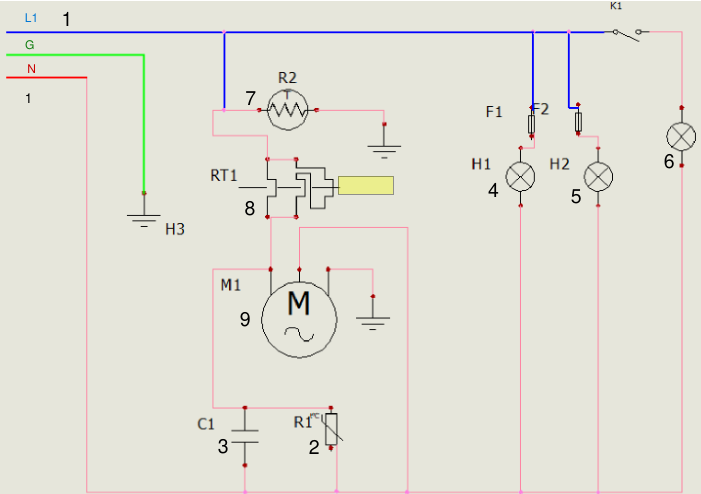
\includegraphics[width=0.7\linewidth]{figures/4-diag-electrico}
	\caption{Diagrama eléctrico}
	Fuente: Elaboración propia en Proteus 8.2
	\label{fig:4-diag-electrico}	
\end{figure}

 \newpage

\section{Conclusión}


La redacción de este capítulo ha sido fundamental en la propuesta de solución para el diseño y selección de componentes de una cámara de refrigeración destinada a la conservación de insulina, especializada en pacientes diabéticos de la alcaldía Azcapotzalco en la Ciudad de México. Conocer y estructurar correctamente las cargas térmicas ha sido esencial para garantizar que el sistema de refrigeración se ajuste de manera precisa a los requisitos de conservación de la insulina, tomando en cuenta las condiciones climáticas específicas de la zona. 

Este proceso ha permitido prever las variaciones de temperatura externas y cómo estas afectan la operación del sistema, asegurando que la insulina mantenga sus propiedades farmacológicas y su eficacia durante todo su periodo de almacenamiento. La correcta estimación y estructuración de las cargas térmicas es crucial para diseñar un sistema de refrigeración que no solo cumpla con los estándares de conservación, sino que también sea eficiente en términos energéticos, reduciendo costos operativos y minimizando el impacto ambiental.

Finalmente, la eficiencia en la conservación de insulina en los hospitales públicos de la Ciudad de México es de vital importancia para garantizar el bienestar de los pacientes diabéticos, especialmente en zonas de alta demanda como Azcapotzalco. El correcto funcionamiento de estos sistemas permitirá evitar el deterioro de la insulina, asegurando un suministro constante y seguro para los pacientes que dependen de ella.



